% -----------
% SETUP
% -----------
\documentclass{physics_article_B}
\title{Mechanical Vibrations of Droplets in Fluidic Systems}
\mytitle{Mechanical Vibrations of Droplets in Fluidic Systems}
\myname{Dominic Coy \& Oliver Gordon}
\studentid{4227789 \& 4224942}
\date{Due Date: 1 June 2018}
\setlength{\bibsep}{10pt plus 0.3ex}
\begin{document}
	
% ----------------------
% COVERSHEET
% ----------------------
\pagenumbering{roman} 
\setcounter{page}{0}
%\includepdf[scale=1]{Images/Cover.pdf}
%\maketitle

% ----------------------
% ABSTRACT
% ----------------------
\pagenumbering{gobble} 
\begin{abstract}
	\large{Insert the geratest abstract ever written 
}
\end{abstract}
	
% ----------------------
% CONTENTS
% ----------------------
%\vspace{4cm}

\tableofcontents

\pagenumbering{roman} 
\setcounter{page}{1}
\setlength{\parskip}{6pt}  
% ----------------------
% INTRODUCTION
% ----------------------
\newpage
\pagenumbering{arabic} 
\setcounter{page}{1}

\section{Introduction\label{sect:intro}}

    Simultaneously measuring the rheological properties of fluids, such as viscosity and surface tension, has, in the past, been accomplished with rheometers or drop volume. However, these methods are not particularly viable when analysing rare or expensive liquids such as blood droplets in forensics. When only a few millilitres of fluid are avaliable, the most promising analysis method is to induce oscillations in small droplets\textsuperscript{\cite{harrold}}, and detect these vibrations with a laser. Other applications of this vibrational method and supporting theory include monitoring inkjet printing performance\cite{Martin2008}, simulating the crustal deformation of planets\cite{vukasinovic}, and studying energy relaxation in stars\cite{vukasinovic}.
    
    Early experiments using droplets were based on theoretical models developed by Rayleigh\textsuperscript{\cite{rayleigh}} and Chandrasekhar\textsuperscript{\cite{chandrasekhar2}} who showed that, by using simple equations, vibrational frequencies of droplets were related to the viscosity and surface tension of a free liquid globe (essentially a levitated droplet). Temperton et al. claimed to be the first to present a combined theoretical and experimental study of simple Newtonian fluids (such as water) in 2014\textsuperscript{\cite{temperton}}. This approach was later extended by multiple authors who demonstrated that, provided surface tension is already known, the technique could be used to extract frequency dependent physical properties of viscoelastic droplets (such as blood)\textsuperscript{\cite{egry}}. 
    
    Although multiple previous authors have demonstrated the viability of manual testing, this is not ideal for obvious reasons. As such, we aim to develop a proof of concept system to automate this process. This will involve building a high-throughput system to consistently create and transport spherical droplets suspended in oil. The droplets can then be oscillated and analysed, with a laser and photodiode, to determine their rheological properties.
    
    Once the potential to automatically probe droplets has been demonstrated, one of the largest remaining issues involves incomplete theory. Although the droplets investigated here are simple Newtonian fluids such as water, in future viscoelastic materials, such as blood, could be investigated. Building on the ability to track properties of a fluid in real time by Harrold et al. in 2016\cite{harrold}, this could be applied to lab-on-a-chip systems, such as inexpensive, reliable tests\textsuperscript{\cite{yager}} for medical diagnosis. Furthermore, droplets containing mixed fluids could also be investigated, and so could the interfacial tension between two liquids\textsuperscript{\cite{Backholm2017}} simultaneously.
    
    In this paper we begin by discussing the history of the field and associated theory, before discussing the computer vision techniques used to determine droplet size. We then discuss the multiple methods with which we attempted to induce and detect oscillations, and explain how the system was automated. We then briefly demonstrate the validity of this system with distilled water, before discussing our results and their implications. Finally, we discuss future improvements to the project and indicate future directions to the research.

% ----------------------
% Literature Review
% ----------------------
\newpage
\section{Literature Review\label{sect:lit}}

    Building on the work by Rayleigh in 1879, which related the frequency of oscillation of fluidic jets with their area and pressure\textsuperscript{\cite{rayleigh}}, in 1932 Lamb et al. derived an expression for the oscillation frequency of inviscid droplets in an inviscid fluid. They also derived approximate expressions for the rate of damping of oscillations in a viscous droplet in an inviscid fluid and for the oscillations of a bubble of gas in a low viscosity liquid. In their derivations, the velocity fields found for small oscillations of an inviscid fluid were used to estimate the rate of viscous dissipation (rate that shear forces turn work done by a fluid on adjacent layers into heat) in a droplet with small viscosity\textsuperscript{\cite{lamb}}. Then, in 1960, Reid analysed the oscillations of a viscous droplet in a low-density gas or a vacuum\textsuperscript{\cite{reid}}. His experiment and analysis were summarised in the book Hydrodynamics and Hydrodynamic Stability by Chandrasekhar in 1961\textsuperscript{\cite{chandrasekhar}}. In 1965, Velentine et al. used the same methods as Lamb et al. to derive expressions for the damping rate of oscillations when a low viscosity droplet was submerged in a low viscosity fluid\textsuperscript{\cite{velentine}}. In 1968, Miller et al. derived a general dispersion equation for the oscillations of viscous droplets immersed in a viscous fluid, which could also be applied when the interface between the two fluids possessed elastic and viscous properties of its own. They also derived equations for the rate of damping of oscillations and frequency for specific cases including when the interface between the two fluids is free or is inextensible\textsuperscript{\cite{miller}}.
    
    
    Over the years, experiments have focused on a variety of droplet shapes. Two of the three common droplet geometries are sessile (suspended on a surface)\cite{Temperton2012, vukasinovic, Backholm2017} and pendant (teardrop-shaped and suspended off a surface such as a needle)\cite{Temperton2012}. Despite the relative experimental ease of investigating these suspended droplets, damping interactions and droplet shape can be influenced by the suspension surface or the pipette used to transport them\cite{Sharp2011}. This alters the vibrational spectra, producing errors yet to be fully rectified\cite{harrold}. Despite this, many authors limit such experiments to a single surface\cite{Sharp2011}, leading to differing results. These mechanisms can be avoided using either superhydrophobic or superamphiphobic surfaces as the droplets take on a spherical shape and can be described with similar equations to levitated droplets.
    
    Much of the initial research within this area looks to have been driven by the ambition to study containerless crystallisation of pure liquids in microgravity\textsuperscript{\cite{wilkes}}. Although it is possible to investigate large spherical droplets by performing the experiment in low gravity (as done in 1979\cite{holt} on Space Shuttle Columbia), this is obviously impractical for our purposes. As such, many recent experiments have analysed levitated droplets using various different methods. Methods that have been used to levitate the droplets include magnetic\textsuperscript{\cite{hill}}, electrostatic\textsuperscript{\cite{mugele}}, acoustic\textsuperscript{\cite{trinh}} and aerodynamic\textsuperscript{\cite{benmore}}. McHale et al. demonstrated the feasibility of this method using vibrating liquid marbles (droplets stabilised by the adsorption of small particles). However, they found that the small particles dominated the droplet's physical properties and so the application of this approach is limited\textsuperscript{\cite{mchale}}. Hence, there is a great interest in analysing droplets suspended within another fluid. 
    
    One of the main advantages of fluidic levitation involves lower mass loss. During an experiment, mass will be lost as the droplet evaporates over time. For fluidic levitation, this has been shown to be 2-4\%, which is significantly lower than for other methods which see over 10\% \cite{harrold2} mass loss. However, to the best of our knowledge no author has modelled this mass loss and taken it into account. Furthermore, the way in which mass is calculated is also very basic; the droplet is weighed before and after an experiment by comparing the mass of a syringe or paper towel both with and without the droplet. These methods do not take into account leftover residue, and in the case of paper towels are destructive. Additionally, this method of levitation requires placing droplets by hand, which is a slow process. There is therefore a significant impetus to develop a high throughput system allowing multiple droplets to be quickly analysed in a hands-off fashion.
    
    As such, we intend to investigate the other common droplet shape of spherical droplets. These are formed by levitating fluid away from a surface using methods such as magnetic\cite{temperton, hill}, electrostatic\cite{mugele, wong}, aerodynamic\cite{benmore}, acoustic\cite{Temperton2012, Yarin1998}, and fluidic levitation. Fluidic levitation is achieved by placing a droplet of fluid within a suspension medium of different viscosity. Besides spherical droplets, sessile droplets can also be investigated in this fashion by placing them on a suspension slide, as recently demonstrated by Backholm et al\cite{Backholm2017}. These authors also showed that\cite{Backholm2017} by using fluidic levitation, it is possible to determine both the interfacial tension between the droplet and the surrounding liquid, and the rheological properties of the surrounding liquid. %This last sentence is also in the introduction consider removing

\section{Theory\label{sect:theory}}

    As we assume that the droplet remains at constant volume, only liquids can be explored as they are incompressible.

    Following on from prior work, we will be making the major assumption that our droplets will be perfectly spherical. The lowest energy state (and therefore shape) of a droplet is influenced by its surface tension, $\gamma$, and gravitational interactions, $g_{eff}$. $\gamma$ makes the droplet spherical, whilst $g_{eff}$ distorts it. Because these two interactions oppose each other, there exists a critical droplet radius at which its shape changes from spherical to distorted. This is known as the capillary length, $l_{cap}$, and is defined by the equation\cite{temperton},
        
        \begin{equation} 
        \label{eq:lcap}
            l_{cap} = \sqrt{\frac{\gamma }{\rho g_{eff} }}, 
        \end{equation}
    
    where $\rho$ is the density of the droplet. It can therefore be assumed that a droplet is spherical if it has radius, $R$, lower than its capillary length $l_{cap}$. However, as $l_{cap}$ is not always known, it is imperative that droplets are kept as small as possible. 

    Because the droplet has an equilibrium shape, it will undergo shape oscillations when a small perturbation is applied\cite{oscillate}. If this perturbation is in the form of an impulse, the surface of the droplet will be driven at all frequencies (owing to the mathematics of Fourier transforming a delta function). Vibrations not at the resonant frequency are damped, leaving only the vibrations at the resonant frequency of the droplet with a non-zero amplitude. For optimal results, it has been shown that any applied impulse must be long enough to give sufficient time to perturb the drop, but short enough to still be an impulse and not drive the droplet at a particular frequency\cite{temperton}. Furthermore, the amplitude of oscillations must be kept to under 0.1$R$, following work from Becker et al. who found that above this limit oscillations become non-linear, causing the simple equations used here to fail\cite{becker}.
    
    These oscillations decay exponentially, giving a time dependant signal such as the one shown in Figure \ref{fig:temperton:signal}. The power spectral density can then be obtained by fourier transforming this signal, and is demonstrated in Figure \ref{fig:temperton:PD}. The remaining resonant frequencies correspond to different modes, $n$, of oscillation. The $n=1$ node corresponds to oscillations of the droplet's centre of mass\textsuperscript{\cite{miller}}, whilst the $n\geq2$ nodes correspond to the surface oscillations which are of interest here. The corresponding frequency, $f_n$, and full-width-half-maxima, $\Delta f_n$, can then be extracted. 

        \begin{figure}[H]
            \centering
                \begin{subfigure}[b]{0.48\textwidth}\hspace*{-1cm}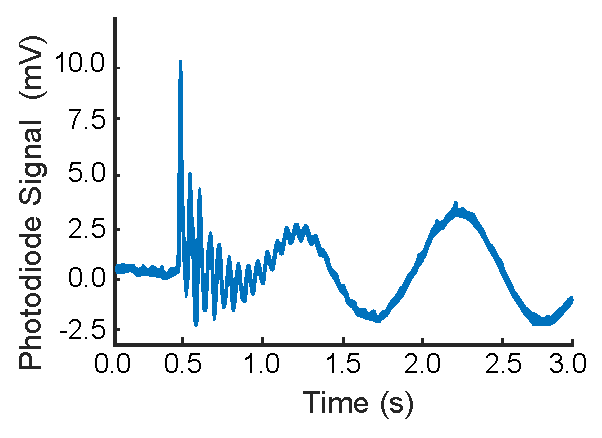
\includegraphics[width=\textwidth]{Figures/TempertonSignal.eps}
                    \caption{Original Signal}
                    \label{fig:temperton:signal}
                \end{subfigure}\hspace{3pt}
                \begin{subfigure}[b]{0.48\textwidth}\hspace*{-0.5cm}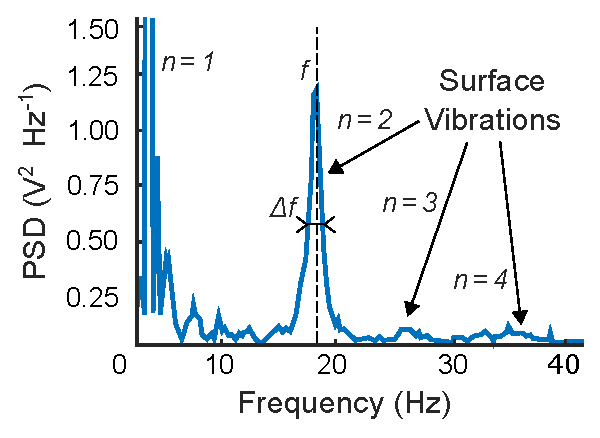
\includegraphics[width=\textwidth]{Figures/TempertonSignalPD.eps}
                    \caption{Fourier Transform}
                    \label{fig:temperton:PD}
                \end{subfigure}
            \caption{Figure to demonstrate (a) the time dependant signal produced when oscillating a droplet of water with an impulse, and (b) its resulting fourier transform. The resonant vibrations on the surface of the droplet can be seen in (a) as the initial, rapidly oscillating components of the signal. These correspond to multiple nodes, $n$, of oscillation in (b). The frequency, $f$, and full-width-half-maxima, $\Delta f$, can then be used to determine the rheological properties of the droplet. }\label{fig:temperton}
        \end{figure}

    The surface tension, $\gamma$, and viscosity, $\eta$, of the fluid can then be calculated using the equations,
 
        \begin{equation} 
        \label{eq:SurfaceTension}
            \gamma = \frac{4\rho R^{2}}{\pi n^{2}}(\Delta f^{2} + f^{2}),
        \end{equation}
        
        \begin{equation} 
        \label{eq:Viscosity}
            \eta = \frac{\pi \rho \Delta f R^{2}}{n^{2}},
        \end{equation}

    where $\rho$ is the density of the droplet. To determine $R$, checkerboards of known dimensions can be used to map the pixels on a screen to real world space. Because cameras have no depth-perception, this requires the assumption that the object of interest is in the same plane as the checkerboard. Once the height and width of a spherical droplet, $R_x$ and $R_y$ respectively, has been found in an image containing a checkerboard, $R$ can be calculated with simple trigonometry,
            
        \begin{equation}\label{eq:radii}
            r = \sqrt{\Big(\frac{R_x}{2}\Big)^2 + \Big(\frac{R_y}{2}\Big)^2} .
        \end{equation}

    However, Equations \ref{eq:SurfaceTension} and \ref{eq:Viscosity} are only valid for simple Newtonian droplets such as water and glycerol. For viscoelastic droplets such as amorphous polymers, biopolymers, metals at very high temperatures or bitumen materials, there has yet to be a complete analysis of droplets without prior knowledge of $\gamma$.
% ----------------------
% Equipment
% ----------------------
\newpage
\section{Methods\label{sect:method}}

    \subsection{Slide \& Fluid Loop\label{sect:method:slide}}
    
        To interrogate liquids of interest, a clean test environment had to be created. This was accomplished by first creating a plastic mould with a 2 mm diameter tunnel inside. This ensured that all droplets were well below the 2.7 mm capillary length of water\cite{capillary}. The mould was then filled with PDMS, placed on a glass slide and cured. A 1 mm port was also created on the top side of the slide, and subsequently used to inject fluids of interest. This smaller diameter was chosen as the higher pressure it created prevented backflow/droplets constantly flowing when only a single droplet was ever desired in the slide at any one time.
        
        Three capillary tubes were then attached these ports, before sealing all leaks with flowable silicon. This setup is demonstrated in Figure \ref{fig:control}. Because of the difficulties and long drying times involved with manufacturing perfectly sealed PDMS slides with smooth tunnels, we later changed to perspex instead of glass/PDMS, and carefully drilling the appropriate holes. This had the advantage of being quicker to produce, less fragile, and less prone to internal leaking. 
        
            \begin{figure}[H]
                \centering
                    \hspace*{2.4cm}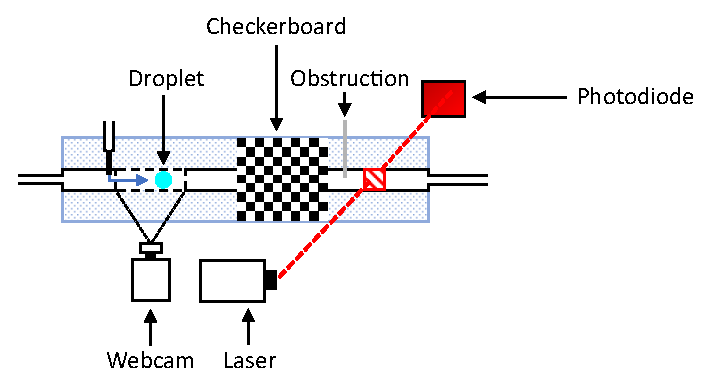
\includegraphics[scale=0.9]{Figures/Control.eps}
                    \caption{Figure to demonstrate the sealed chamber used to investigate continuously moving droplets. Into a slide consisting of PDMS, a cylindrical tunnel was created. Droplets were injected through the top port and flowed from left to right. After photographing a calibration checkerboard with a webcam, a small slice of this tunnel was selected and continuously monitored, and the size of passing droplets determined. The droplet was then oscillated with a variety of methods (in this case a small obstruction). Oscillations caused a laser beam directed at the tunnel to disperse, which was then detected with a photodiode.} 
                \label{fig:slide}
            \end{figure} 
    
        To move droplets through the slide, the capillary tubes were then connected to a fluid loop consisting of 3 mm tubes. To transport the spherical droplets, mineral oil of a lower viscosity was used as a carrier medium. A microfluidics motor was used to transport the oil from a central reservoir and around the loop. To reduce stress on the capillary tubes of the slide, the motor was attached on the "in" side, so oil is not being pulled against the external tubes, potentially breaking them (?). A t-junction was also placed at the return side of the loop to allow for easy bleeding of air. Droplets were injected into the 1 mm port with a motorised syringe. After being interrogated in the slide, droplets were transported to the reservoir. Here, they could be easily removed by hand, as the droplets were of different density to the mineral oil, so would either sink or float. To prevent these droplets from returning into the flow system, the return and collection tubes were placed at different heights on opposite sides of the reservoir. This setup is demonstrated in Figure \ref{fig:basic}.
        
            \begin{figure}[H]
                \centering
                    \hspace*{2.0cm}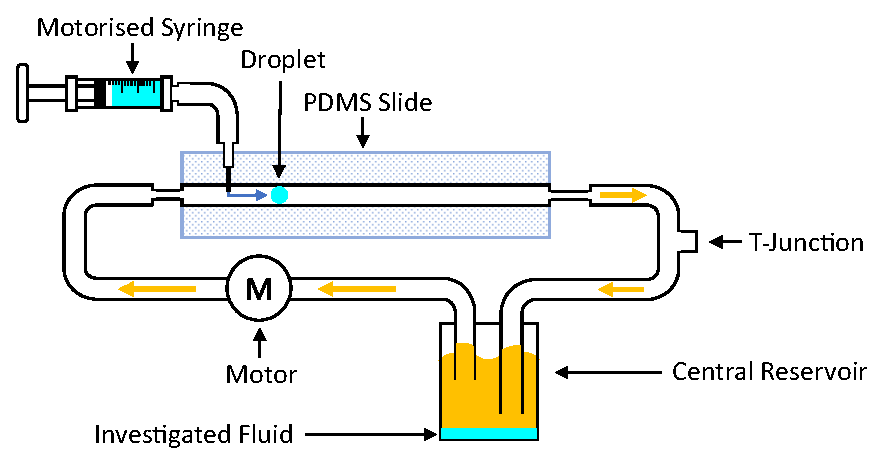
\includegraphics[scale=0.8]{Figures/Fluid.eps}
                    \caption{Figure to demonstrate the flow circuit used to investigate the rheological properties of droplets. Using a motor, a suspension fluid of mineral oil was transported from a central reservoir to a PDMS testing environment and back. A t-junction was placed in the back half of the loop to bleed air out of the system. A motorised syringe was used to suspend droplets of interest in the mineral oil, and subsequently investigated inside the PDMS slide. Droplets were then transported back to the reservoir, where they could be retrieved.} 	
                \label{fig:basic}
            \end{figure} 

    \subsection{Motor \& Syringe Pump\label{sect:method:motor}}

        To allow the speed of the fluid to programmatically controlled as part of the computer vision system described below, the motor had to be driven by a DAQ card. However, the card used lacked the circuitry to output sufficient current, making it unable to turn the motor at any voltage. Furthermore, the card had poor output resolution, making very fine control of fluid speed impossible. A current boosting circuit was therefore produced, and is shown in Figure \ref{fig:MotorCircuit}.  
        
            \begin{figure}[H]
                \centering
                \hspace*{-1.8cm}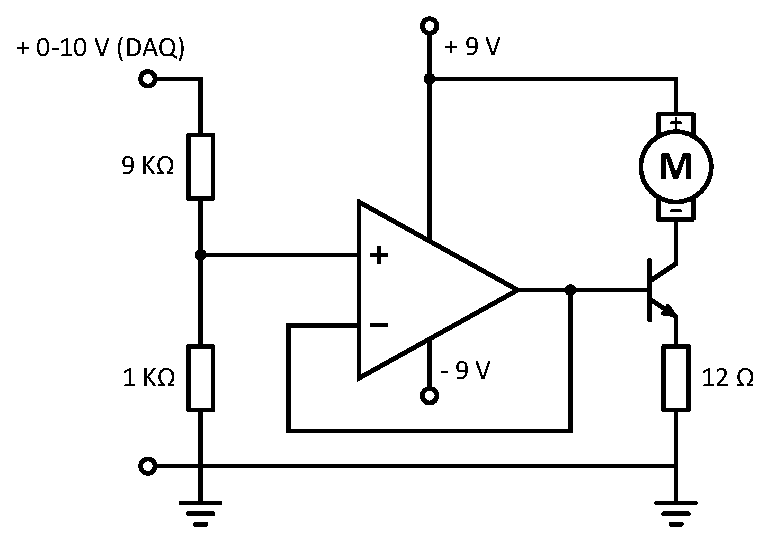
\includegraphics[scale=0.8]{Figures/MotorCircuit.eps}
                \caption{Figure to demonstrate the circuit schematic of a circuit used to programatically control the voltage applied to a motor. Depending on a 0-10 V signal from a DAQ card, between 0-4 V at 0-400 mA could be applied to the motor. This was required as the DAQ card alone was unable to produce sufficient current to drive the motor.}
                \label{fig:MotorCircuit}
            \end{figure}
        
        Besides using an external power supply to increase output current to suitable levels, it maps the 0-4 V input rating of the motor to the full 0-10 V output of the DAQ, effectively increasing its sensitivity. Resistances were chosen both to provide the required output and provide good heat dissipation. Heat dissipation was further improved by attaching a heatsink to the transistor. The 12 $\Omega$ resistor was also replaced with 3 x 36 $\Omega$ resistors to reduce component stress. The motor was given protection by powering the circuit with a current limited power supply set at the maximum current rating of the motor. This is shown in Figure \ref{fig:MotorCalib} where the motor voltage goes up linearly with the DAQ voltage up until a DAQ voltage of 6.0 V and above where the motor voltage is limited to 4.0 V.
        
        To allow droplets of a consistent size of be created, a motorised syringe pump was set up, and code created to automatically interface over a COM port. To decrease the size of droplets being produced, the speed of the motor could be increased. However, droplets needed to be moved as slowly as possible to increase the time of data collection. Droplet size could therefore be made larger by increasing the speed at which the syringe pump was turned by writing code to interface with the pump through a serial port.
        
        
    \subsection{Determining Density\label{sect:method:density}}
    
        We employ a different method for determining density than previous others. Typically, $\rho$ is calculated by using $R$ of each spherical droplet to determine its volume, $V$. The mass of the droplet, $m$, is then measured by absorbing a droplet onto a paper towel and comparing to the mass without the droplet\cite{hill}. This method is both destructive and erroneous by up to 10\%\cite{harrold2} due to mass loss during the experiment. It is also not viable for our purposes, as our droplets are suspended in fluid. 
        Instead of measuring density per droplet, we measure density for the fluid in general. By holding our fluid of interest in a syringe, we can compare the mass of an empty and filled syringe. The volume can be easily determined by reading from the scale of the syringe.
    
        This method has multiple advantages. For one, it is non-destructive, making it more practical for many biological investigations such as protein crystallisation studies\textsuperscript{\cite{zhu}}, cell culture bioreactors\textsuperscript{\cite{konry}}, or any time where an expensive/rare liquid needs to be recovered\cite{Backholm2017}. Further, as the system is self contained and has all measurements taken within seconds, no mass is lost to evaporation. Further, averaging down from larger volumes results in a lower percentage error per droplet, improving the accuracy of $\rho$.
        
    \subsection{Computer Vision\label{sect:method:vision}}
        
        \subsubsection{Acquiring Data\label{sect:method:vision:acquire}}
        
            In order to allow droplets to be analysed in real time, a computer vision control system was developed. A Logitech C920 camera was chosen for its high image quality, high resolution, and wide field of view. 
            
            One of the major difficulties encountered during studies is to quickly compute the radius of droplets. Previous authors typically accomplish this by photographing a perfectly lit droplet, counting the widths of pixels and using trigonometry with the camera focal length. For the case of transparent droplets, automated computer vision is considered extremely difficult. This is in spite of the common requirement of big money industries such as fuel manufacturing to identify and quantify droplets during manufacturing\cite{bubblegeneral}. For one, without perfect, even lighting surrounding the droplet, droplets do not have bright regions of contrast fully around their boundary. In the case of transparent droplets, further difficulties arise due to the centre looking identical to its surrounding. Droplets can also have bright reflections in their middle, further confusing simple algorithms\cite{bubblegeneral}. The inevitable presence of noise in images also adds further complexity. As such, more complex algorithms can take nearly a minute to run, and still only achieve accuracies of approximately 80\%\cite{bubble2} for detecting droplets.

            Because droplets are not static, strict requirements are placed on the efficiency of calculations. Furthermore, as MATLAB is an interpreted language and lacks hardware acceleration, webcam acquisition operates at very low framerates, making tracking moving droplets in real time difficult. This was overcome by modifying Hebicam\cite{HebiCam}, which was originally created for streaming CCTV footage, and is a MATLAB wrapper for the more efficient openCV. After adapting this package for use with USB webcams, 1080p video could be acquired at 30 FPS with spare processor overhead to perform calculations, as opposed to 6 FPS with none. Furthermore, data was acquired in grayscale (as opposed to RGB), further increasing capture efficiency and reducing the size of stored data. 
            
    
        \subsubsection{Calibration\label{sect:method:vision:calib}}

            To ensure that droplet size was calculated accurately, we applied checkerboard calibration using checkers of a known size. An algorithm implemented in MATLAB\cite{CameraCalibration} was then used to calculate various extrinsic properties of the camera, such as the optical centre, distortions, and focal lengths in x and y. 
        
            There was an added complication to this process in that the PDMS used to create the experiment area was not perfectly flat. Because the algorithms work on the assumptions that checkerboard is flat and the droplet is in plane with the checkerboard, the pattern was instead printed on a long piece of paper, carefully folded and tensioned to the back of the slide. However, this resulted in a small 1mm disparity in depth between the droplet and the checkerboard, resulting in a small error. Using simple trigonometry to measure the distance to objects, this error was estimated to result in a 0.05 mm underestimation of all values of $R$, and as such was added to all calculated values of $R$. 
            
            Further, a limitation was placed on the maximum size of the checkerboard because the slide was of a finite size. Larger checkers had a lower percentage error from imperfect focusing, but smaller checkers could be placed in greater numbers. To determine the optimum checkerboard size for our purposes, we calibrated the camera with checkers between 1.50 and 5.00 mm in size and attempted to determine the size of circles of radius 0.10 to 1.00 mm, and accounted for the 0.05 mm offset. 
            
            Ultimately, it was found most optimal to use checkers of size 0.20x0.20 mm in a 10x11 grid. 20 calibration images were then taken at different positions in similar positions to those used during our experiment. The positions of the checkerboard in the calibration screenshots as determined by the algorithm are shown in Figure \ref{fig:calib}. 
            
                \begin{figure}[H]
                    \centering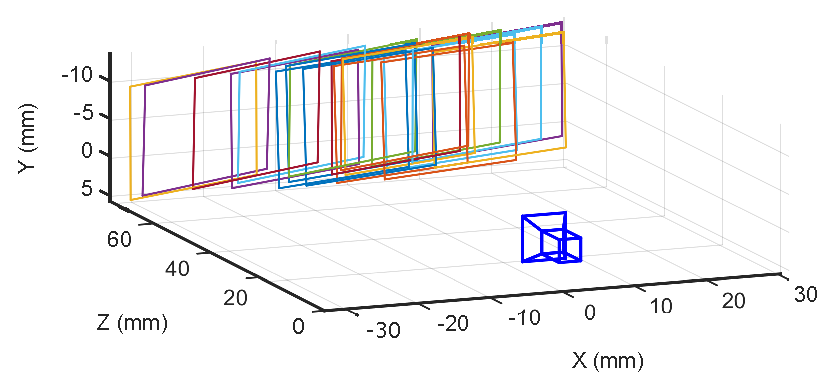
\includegraphics[scale=0.86]{Figures/CameraExtrinsics.eps}
                    \caption{Figure to demonstrate the multiple positions a checkerboard was placed in to calibrate a webcam. By taking multiple pictures of the checkerboard in multiple positions and knowing the size of the square checkers, the camera was be algorithmically calibrated to reliably determine object size. Because the positions of the checkerboard calculated by the algorithm agreed with the real-world placements, the camera was known to be accurately calibrated.}\label{fig:calib}
                \end{figure}
            
        \subsubsection{Determining Droplet Size\label{sect:method:vision:size}}
                
                Because droplets were confined to a small area at any one time, only a small 3 mm long window of the slide was ever observed at one time to improve performance. Because moving droplets would suffer from motion blur, the motor first had to be stopped when a droplet was present within this small window. 
                
                To do this, a background photo of the window was  taken with oil flowing but no droplet present. Every time a frame of video was captured, the window was subtracted from the corresponding background. This allowed differences in pixels to be seen. To increase the contrast of these difference in a non-linear manner, they were multiplied by the arbitrarily selected log(6). When a droplet was present in the window, fully bright regions could be easily seen in the area where the droplet was. Once an arbitrary threshold of bright pixels was reached, the droplet was confirmed as being in the window, and the motor stopped. These steps are demonstrated in Figure \ref{fig:detector}.
            
                    \begin{figure}[H]
                        \centering
                        \begin{subfigure}[b]{0.3\textwidth}
                            
\includegraphics[width=\textwidth]{Figures/DropFinder/DropFinder1.eps}
                            \caption{Background}
                            \label{fig:detector:back}
                        \end{subfigure}
                        ~ 
                        \begin{subfigure}[b]{0.3\textwidth}
                            
\includegraphics[width=\textwidth]{Figures/DropFinder/DropFinder2.eps}
                            \caption{Foreground}
                            \label{fig:detector:fore}
                        \end{subfigure}
                        ~ 
                        \begin{subfigure}[b]{0.3\textwidth}
                            
\includegraphics[width=\textwidth]{Figures/DropFinder/DropFinder3.eps}
                            \caption{Difference}
                            \label{fig:detector:diff}
                        \end{subfigure}
                        \caption{Figure to demonstrate how droplets were detected after being created by a mechanical pump. A region of the webcam was defined, and a background image taken (a). The region was then continuously monitored. If a droplet was present in the region (b), it could be detected by calculating the difference between (b) and (a) and multiplying by a log. If enough bright pixels were observed (c), a droplet was known to be present in the system.}\label{fig:detector}
                    \end{figure}
            
            To reduce motion blur further, the system was thoroughly bled of air at all times. This is because air was the least dense medium present, and as it moved to the highest point in the system it pushed the oil and therefore the droplet. 
            
            Although this logical test based on bright pixel number is sensitive to noise, it was chosen over an object finder as calculations had to be performed in under 1/30 of a second, as otherwise the droplet could pass the window and fail to be detected, causing the entire system to fail. This noise means that the carrier fluid must be single coloured and free of impurities. 
            
            After stopping the motor and waiting for it to spin down, a new photo could be taken of the droplet, which was guaranteed to be in the pre-defined window, and its outline calculated. This was achieved with a 5-stage algorithm. First, the image was subtracted from the background as before to remove background shapes. To bring out fine dark detail and reduce bright noise, a top-hat filter was then used to set all pixels with brightnesses below 10 to 0 (i.e. black), and all pixels with brightnesses above 20 to 255 (i.e. white). Of the remaining data, an automatic binarising algorithm was then applied to further bring out fine detail, and make a solid white horseshoe. This horseshoe was then turned into a convex hull and filled in. This shape could then be assumed to be a circle, and detected with a Circular Hough Transform based algorithm\cite{imfindcircles}. Each stage of the algorithm is shown in Figure \ref{fig:size}.
            
                \begin{figure}[H]
                    \centering
                    \begin{subfigure}[b]{0.3\textwidth}
                        
\includegraphics[width=\textwidth]{Figures/SizeFinder/SizeFinder1.eps}
                        \caption{Raw Image}
                        \label{fig:size:1}
                    \end{subfigure}
                    ~ 
                    \begin{subfigure}[b]{0.3\textwidth}
                        
\includegraphics[width=\textwidth]{Figures/SizeFinder/SizeFinder2.eps}
                        \caption{Background Subtraction}
                        \label{fig:size:2}
                    \end{subfigure}
                    ~ 
                    \begin{subfigure}[b]{0.3\textwidth}
                        
\includegraphics[width=\textwidth]{Figures/SizeFinder/SizeFinder3.eps}
                        \caption{Top Hat}
                        \label{fig:size:3}
                    \end{subfigure}
                
                    \begin{subfigure}[b]{0.3\textwidth}
                        
\includegraphics[width=\textwidth]{Figures/SizeFinder/SizeFinder4.eps}
                        \caption{Binarise}
                        \label{fig:size:4}
                    \end{subfigure}
                    ~ 
                    \begin{subfigure}[b]{0.3\textwidth}
                        
\includegraphics[width=\textwidth]{Figures/SizeFinder/SizeFinder5.eps}
                        \caption{Convex Hull}
                        \label{fig:size:5}
                    \end{subfigure}
                    ~  
                    \begin{subfigure}[b]{0.3\textwidth}
                        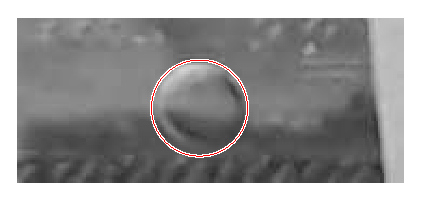
\includegraphics[width=\textwidth]{Figures/SizeFinder/SizeFinder6.eps}
                        \caption{Detected Circle}
                        \label{fig:size:6}
                    \end{subfigure}
                    \caption{Figure }\label{fig:size}
                \end{figure}
            
            After correcting this bounding box for fish-eye in the lens, the height and width, With knowledge of the perimeter of the droplet, a bounding box could be placed around each droplet, pixels converted to mm, and Equation \ref{eq:radii} used to determine the droplet radius.
            
            From this point, the motor could be re-engaged, and the photodiode probed.
    
    \subsection{Oscillating Droplets\label{sect:method:oscillating}}
        
        After determining the size of the droplets, their vibrational spectra had to be determined. It was not possible to follow previous authors and induce vibrations with compressed air as the droplets were contained in a closed system. Magnetic coils were also considered, however this would have limited the approach to magnetic materials. Although the 30 Hz camera recording would not give enough data points to calculate the spectra, it was sufficient to observe oscillations. Vibrations were therefore confirmed to present if they they could be observed by eye with the camera. These were later confirmed with a 360 FPS phone camera.
        
        Multiple methods were attempted to induce oscillations. The first of these methods included the use of a piezoelectric actuators and asymmetrically weighted vibration motors to vibrate the droplet. Secondly, we changed the speed of the motor to pulse rapidly to perturb the droplet. Next we used a DC electric field as it has been shown that a DC pulse passed across an unpolarised droplet can cause it to oscillate. Finally, we used an obstruction in the channel in the form of a copper wire. This made the droplet deform as it clung to the wire causing it to oscillate when freed. We found that for numerous reasons stated in our discussion the obstruction in the channel was the best method to obtain results.
        
    \subsection{Laser \& Photodiode\label{sect:method:laser}}
    
        As the oscillations of the droplet were expected to occur at frequencies higher than the 30 FPS that the webcam could capture at, a photodiode circuit was created to capture the intensity of a laser as it was refracted through the droplet. As our droplets could be assumed to have a different refractive index to that of the carrier oil\cite{viscosity1,viscosity2}, it followed that the presence of a droplet would cause laser light to be scattered differently. Furthermore, as the shape of droplets would vary as the oscillated, they would cause light to scatter in proportion to their degree of oscillation. To observe this effect, a laser was set up as shown in Figure \ref{fig:control}, with the laser on one side of the slide and a photodiode on the other. To prevent 50 Hz noise from an AC-DC power supply, the laser was driven by batteries.
        
        Because droplets would be moving as they oscillated, the laser was focused on a wide area of the slide. However, because the laser was brightest about its focal point, the system would be more sensitive around this region than others. To improve the region of sensitivity, the solid angle of this bright region was increased by setting the laser up at a glancing angle of over 45$^{\circ}$ to the slide, instead of face on. For this reason the laser was later replaced with a wider, more powerful He-Ne laser.
        
        To amplify the output of the photodiode, a simple circuit was set up\cite{artofelectronics}. The variable resistor was used to act as a gain control, allowing the output voltage to be made as high as possible within the recording range of the DAQ card. The 200 pF capacitor was not originally included, but was later added to reduce noise. A larger capacitor reduces more noise, but makes the circuit less sensitive to small changes (i.e. oscillations).
    
        \begin{figure}[H]
            \centering
            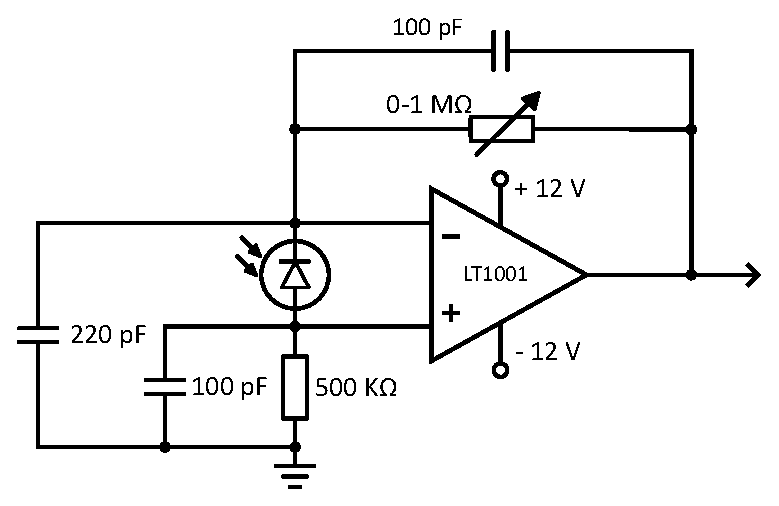
\includegraphics[scale=0.8]{Figures/PDCircuit.eps}
            \caption{Caption}
            \label{fig:my_label}
        \end{figure}
    

    \subsection{Running Experiments\label{sect:method:exp}}
        
        Droplets could be rapidly interrogated through the running of a user-friendly toolbox, which required minimum setup. To set up the code and equipment, files and folders were first created to store raw data. At this point, a previous camera calibration could be selected, or if so desired a new one created with a chooseable number of images. After approving this calibration, operating parameters such as motor voltage and photodiode recording time were then defined. The DAQ card, pump and webcam were then interfaced with so they could be controlled. At this point, the camera was imaged, the checkerboard found, and camera extrinsics calculated. The window of the webcam image in which the droplet was to be imaged was then selected. These steps are shown in Figure \ref{fig:setup:flow}.
        
        \newpage
        \begin{figure}[H]
            \centering
            \hspace*{-5.4cm}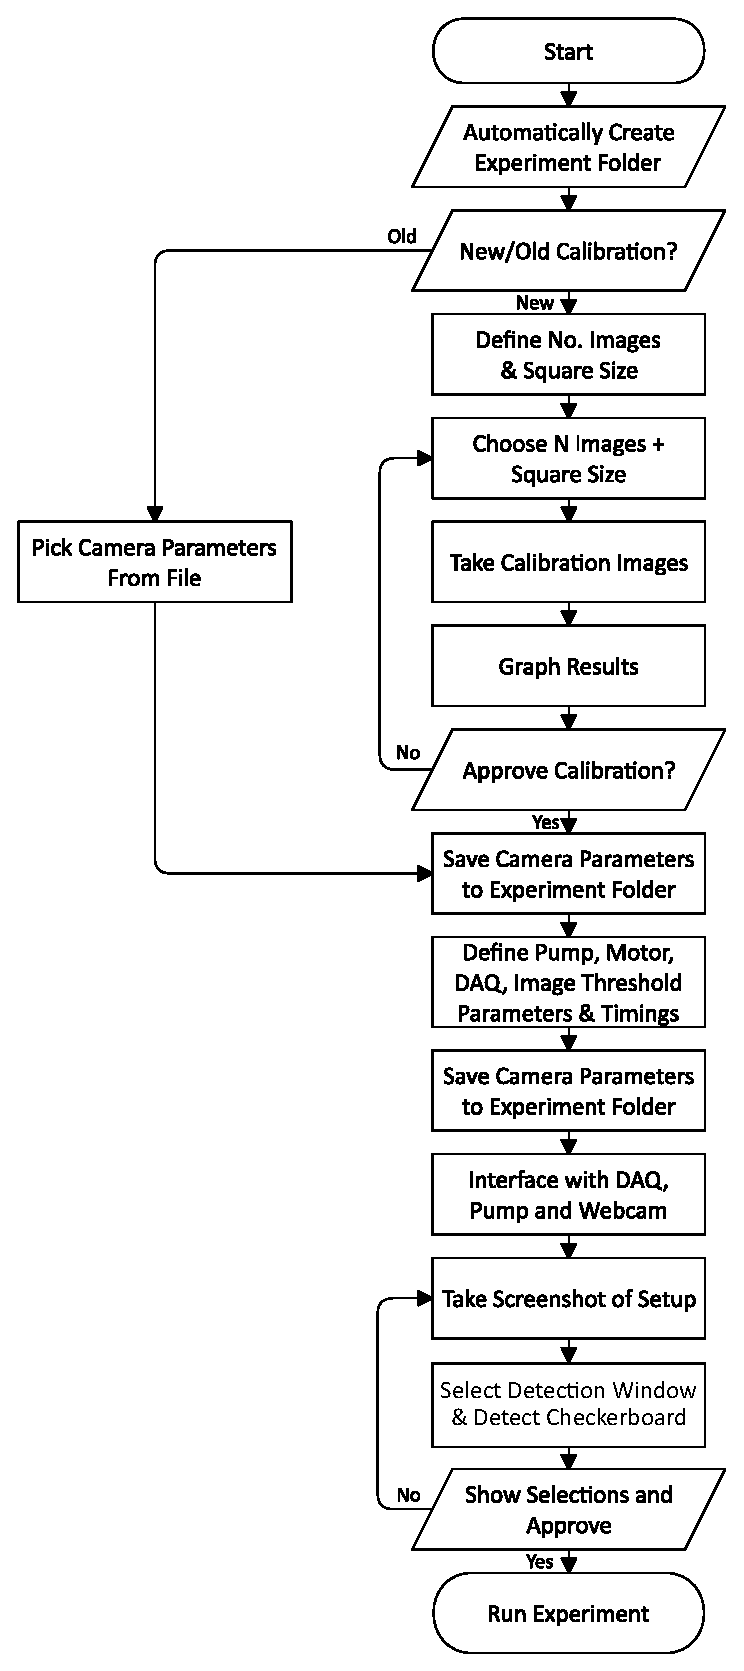
\includegraphics[scale=0.8]{Figures/FlowSetup.eps}
            \caption{Caption}
            \label{fig:setup:flow}
        \end{figure}
        
        From here, no further user input was required, and experiments could be automatically run. As shown in Figure \ref{fig:setup:logic}, this first began with turning on the motor and running it for a few seconds to clear out any stray material from the slide. The detection window defined earlier was then imaged, and the background image shown in Figure \ref{fig:detector:back} taken. The syringe pump was then turned on for just long enough to produce a single droplet of a consistent size. A video was then taken of the window in real time, and after every frame the foreground was subtracted from the background and compared. Once the threshold conditions described in Section \ref{sect:method:vision:size} were met, the motor was stopped, and the size of the droplet found. The motor was then re-engaged, and the photodiode spectrum recorded. After a pre-defined amount of time, oscillations were detected in this spectrum by looking for significant changes in the signal, and this area fourier transformed. The fourier transform could then be calculated, along with $f$ and $\Delta f$. This data was then saved to disk. Further droplets could then be produced to produce further results.
    
        \begin{figure}[H]
            \centering
            \hspace*{-1cm}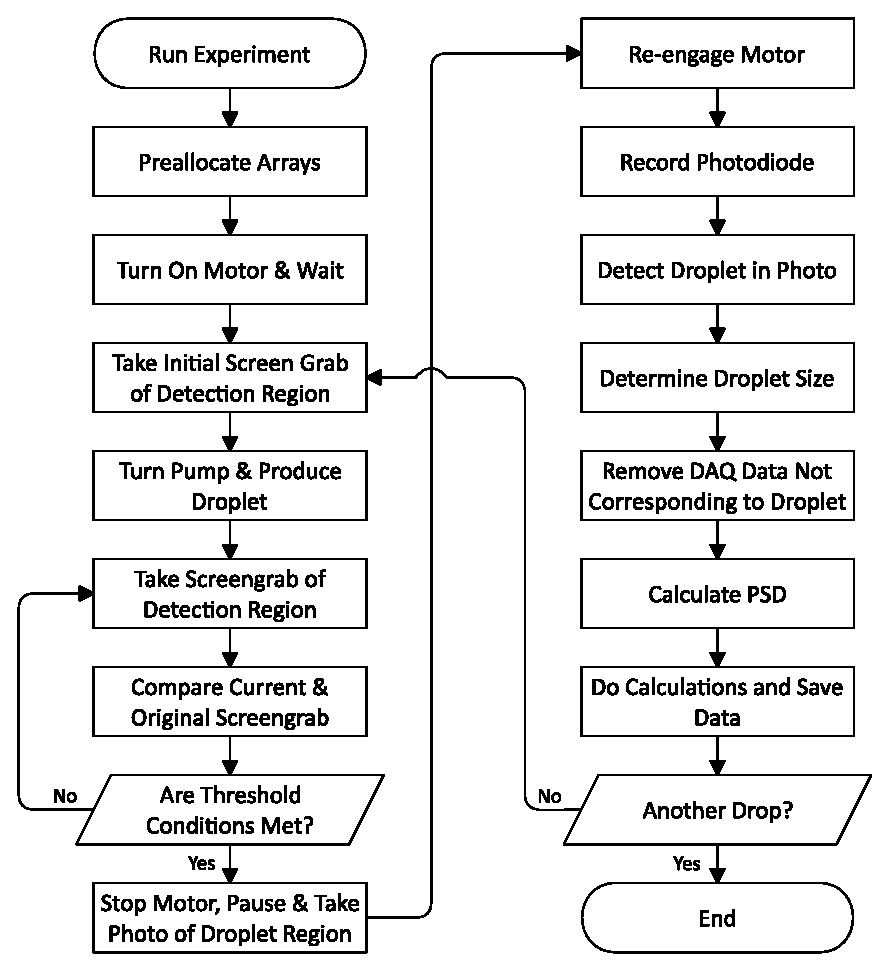
\includegraphics[scale=0.8]{Figures/FlowLogic.eps}
            \caption{Caption}
            \label{fig:setup:logic}
        \end{figure}

\section{Error Analysis} 
    
    There were several major sources of error in the experiment. Firstly, several errors were introduced when determining $\rho$. When the mass of the liquid was calculated by determining the difference in mass of a full and empty syringe, the precision of the measuring scale, 0.001 g was added in quadrature with itself. The corresponding volume of the syringe also had an error from the precision of the scale, 0.2 mL. These two errors were propagated to determine the error on $\rho$.
    
    Furthermore, there were several errors produced when $R$ of the droplets. For one, there was an error due to the imperfect finding of bounding boxes around the droplet. By comparing the diameter of 20 droplets of approximately fixed size when determined both by hand and by algorithm to the nearest pixel, 100\% of the droplets were detected by the algorithm to within 4 pixels in diameter. Given that the diameter of the 2mm thick channel corresponded to approximately 80 pixels, it can be estimated that the boundary of a droplet can be calculated to within 5\% error. This 5\% was then added in quadrature with the error due to imperfect calibrating of the camera. Across the 20 calibration images, there was a mean error of 0.41 pixels (approximately 1 um). The small standard deviation of Y indicated that the calibration was done to a high quality. When calculating the size of known objects, this resulted in an average error of 0.03 mm. This is shown in Figure \ref{fig:calib:error}. 
        
            \begin{figure}[H]
                \centering
                \hspace*{-1cm}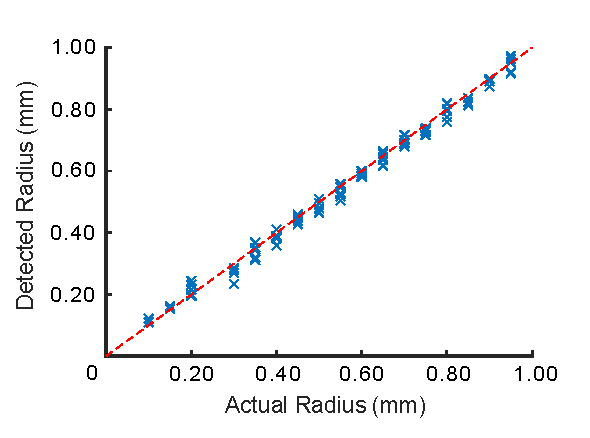
\includegraphics{Figures/CameraCalib.eps}
                \caption{Caption}
                \label{fig:calib:error}
            \end{figure}
    
    The errors on $f$ and $\Delta f$ were also considered. These were defined as the precision of the frequency axis of the fourier transformed signal. To reduce the frequency step in a fourier transform and therefore decrease the errors, both the time of the signal and the sampling rate can be increased. A maximum bound was therefore set based on the maximum time that the droplets would oscillate. Although the DAQ card could theoretically sample at higher than the 2000 Hz experiments were sampled at, various errors occurred when attempting to do so.
    
    Ultimately, the errors on $\rho, R, f$ and $\Delta f$ were propagated through Equations \ref{eq:Viscosity} and \ref{eq:SurfaceTension} to calculate final errors.
    
\section{Results \& Discussion}
    
    \subsection{Control Equipment}
    
        The motor agrees with its rated values (cite).
    
		\begin{figure}[H]
        \centering
        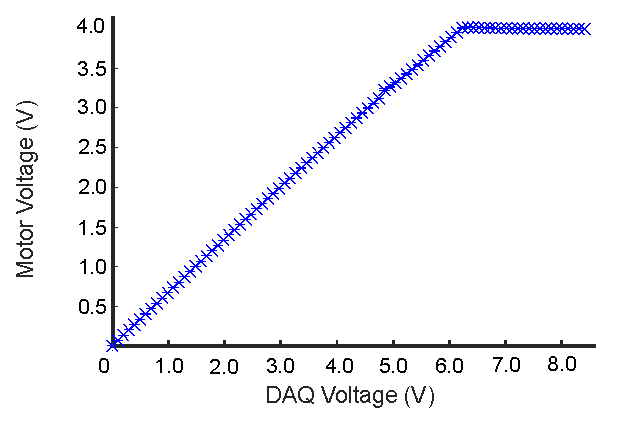
\includegraphics{Figures/MotorCalib.eps}
        \captionsetup{justification=centering}
        \caption{Words.} 	
        \label{fig:MotorCalib}
        \end{figure} 
        
     	From here, it can clearly be seen that the algorithm works as intended (more words)

    \subsection{Oscillating Droplets}
      
        To try and oscillate the droplets we tried 4 different methods. We found that using an obstruction in the channel to perturb the droplets was the best method for us to obtain results. However, we initially considered the use of piezoelectric actuators and asymmetrically weighted vibration motors. As these had to be attached externally to the slide, they therefore made the slide as a whole vibrate and not the droplet contained within. Hence, any oscillations of the droplets were not detectable over the noise coming from the entire slide also vibrating.
        
        From here, we attempted to induce oscillations by changing the speed of the motor using the control circuitry shown in Figure \ref{fig:MotorCircuit}. Although the motor could have been pulsed rapidly, this was akin to driving the droplets at a single frequency, rather than applying an impulse. This was confirmed by the presence of a single peak at the frequency that we were pulsing the motor. Instead, oscillations were attempted to be induced by applying one sudden change in motor voltage, with the hope of having the sudden change in velocity cause the droplet to stretch horizontally and therefore inducing oscillations. This was unsuccessful as the applied force by the change of velocity was too weak to induce any measurable oscillations. 
        
        Next, a DC electric field was considered. For reasons not thoroughly understood in any paper, it has been shown that a short, high voltage DC pulse passed across an unpolarised droplet can cause it to oscillate. A 0-6 kV power supply was therefore introduced. As such, two exposed wires were dug into the PDMS on either side of the fluid channel, and each wire connected to either side of the power supply to set up a simple circuit. To maximise the strength of the electric field, the wires were dug into the PDMS as close to the fluid channel as possible. Because of the high breakdown voltage of PDMS\cite{PDMSBreakdown} of 6 kV mm$^{-1}$, the electric field would be highly localised and directly through the channel. As the droplets moved through the channel and therefore through the field, they would therefore be subject to a DC impulse. This allowed the power supply to be left on at all times, which was necessary as no equipment was available to switch the supply in the oscillation timescales seen in Figure X. To reduce the wires producing stray magnetic fields and causing interference in the photodiode circuit by Lenz Law, all wires were tightly twisted in pairs. The photodiode circuit was also recreated to fit the small size of a grounded metal box. While reducing the noise, created by the electric field, the amplitude of noise for an electric field strong enough to perturb the droplet was too large to detect the oscillations of the droplets.
        
        This noise is shown in Figure \ref{fig:control}. It can be seen from this graph that the electric field voltage is directly proportional to the standard deviation of the photodiode signal. The maximum amplitudes of the oscillations observed were 0.8 V and hence, the noise from the power supply was far too large to be able to consider using the DC electric field as an option as we needed an electric field voltage of over 3.0 kV to see any visible oscillations. 
        
        
\begin{figure}[H]
\centering
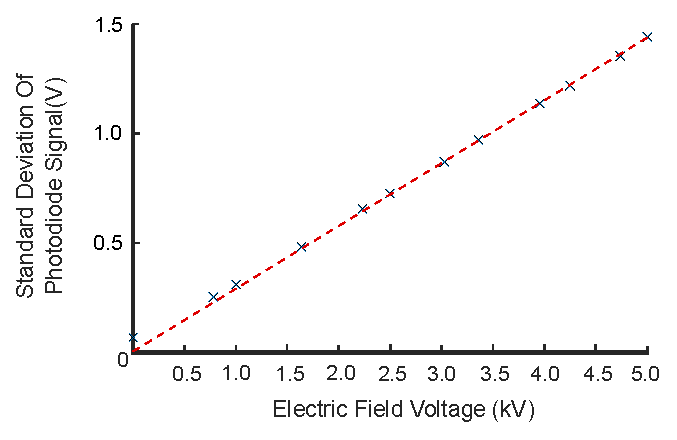
\includegraphics{Figures/ElecFieldNoise.eps}
\captionsetup{justification=centering}
\caption{Words.} 	
\label{fig:control}
\end{figure} 
        
        Finally, a wire obstruction was pushed into the slide. This is shown in Figure \ref{fig:slide}. This method relies on water having a high surface tension of around 70 mNm-1. Water based droplets, amongst others, would therefore be inclined to cling to a new surface when brought nearby. The mineral oil, with a much lower surface tension of around 30 mNm-1, would not. This clinging is demonstrated in Figure X. However, as the droplet moved further away from the obstruction, its equilibrium would once again change to being spherical, and upon "pinging" back to this shape, would begin to oscillate. To increase the strength of the "ping," the droplet was made to cling more strongly to the obstruction by increasing its surface area with sandpaper, and oxidising the surface. Furthermore, a Van-der-Graff generator was also considered to polarise the obstruction, increasing attraction strength further. However, applying a charge when the droplet was nearby caused the droplet to break apart, and because the speed of droplets could never be known precisely, introducing timing circuits for the dissipation of charge would be highly unreliable at best. The height of the obstruction also had to be considered. When the obstruction was deeper into the channel, droplets would be more likely to break up, whilst shallower obstructions would result in oscillations of lower magnitude. As the wire obstruction created the most consistent oscillations with the smallest amount of noise, this is the method that we used to get our results.
 
 	\subsection{Water}
 	
        To determine an idea of the frequency that we expected for our water droplets we conducted an experiment with a sessile water droplet. We softly blew on our droplet to give it the impulse needed to start oscillating. It can be seen from Figure \ref{fig:Water} that once we blew on the droplet there were clear oscillations for around 2 seconds. Once Fourier Transformed we observed that the oscillations were at a frequency of X Hz. From this we knew that we were expecting a similar frequency for our water droplets suspended in mineral oil. This experiment also confirmed that our set up was working as expected as this gave very similar results to X (Temperton) paper. 
 
\begin{figure}[H]
\centering
\begin{subfigure}[b]{0.48\textwidth}                \hspace*{-1cm}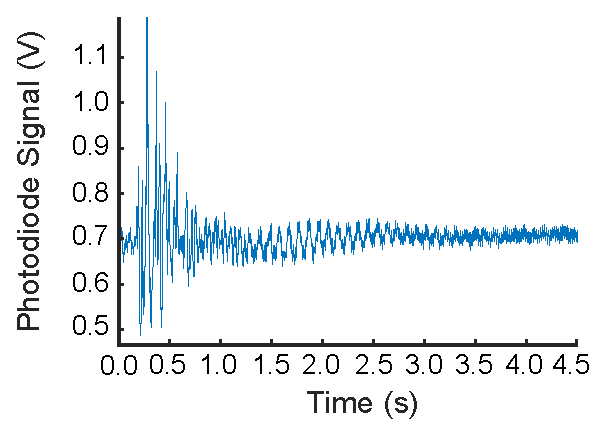
\includegraphics[width=\textwidth]{Figures/WaterSignal.eps}
\caption{Background}
\label{fig:Water}
\end{subfigure}\hspace{3pt}
\begin{subfigure}[b]{0.48\textwidth} \hspace*{-0.5cm}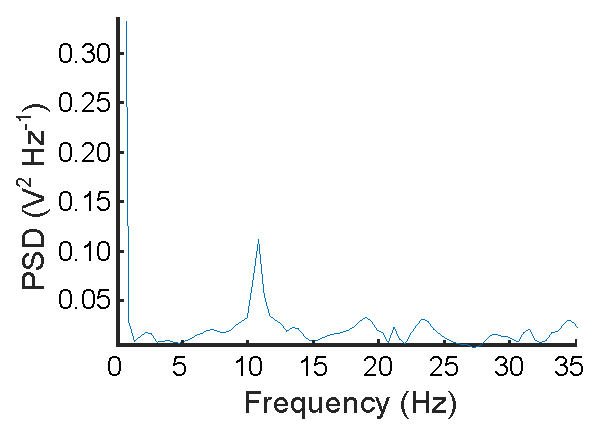
\includegraphics[width=\textwidth]{Figures/WaterSignalPD.eps}
\caption{Foreground}
\label{fig:detector:test}
\end{subfigure}
\caption{Test}\label{fig:test}
\end{figure}
    
\section{Limitations \& Future Improvements}

Some limitation of our project included that our MatLab code was written to automatically interface with the pump over a COM port. This has a significant delay, reducing the throughput of droplets in our system.

There are a few drawbacks to this algorithm. For one, it is highly sensitive to noise, meaning that if the oil is cloudy then it will fail. The top-hat filter is also semi-manual, and must be tweaked for different droplet colours/transparencies. It also struggles with droplets with a radius below 0.3 mm. Finally, it also relies on our assumption that the droplets are perfectly spherical, which is not completely true.

One error that future studies will  have to try and improve is our error on the detected size of the droplets. This error is largely due to the pixel-level precision and small number of pixels taken up by the droplet. As the droplets produced for the experiment were typically around 25 pixels in radius, they only took up 2000 of the 2073600 pixels in a 1920 x 1080 image, only around 0.1\% of the pixels of the image. If the camera had a lower focal length it could be positioned far closer to the droplet, allowing droplets to take up a higher percentage of the pixels in the image allowing for much better image detection and hence, a much smaller error in the droplet size calculator. Another method to decrease this error would be to use a higher resolution camera as it would also increase the accuracy of boundary detection due to the larger number of pixels detected in the droplet. 

As we have shown that droplets can be made to reliably oscillate using our system, future work should focus around refining methods to observe these oscillations. Some methods that could be used to observe these oscillations with more ease include using either a more powerful laser or one with a much wider beam. This would allow oscillations to be observed with a greater amplitude, in the case of a more powerful laser, or for a longer period of time, for a wider beam. Another method that could be used to detect oscillations for longer periods of time is to use either a larger photodiode or a wide array of photodiodes and add up the signal from each one. A avalanche photodiode could also be used to be even more sensitive to the variations in the signal related to the oscillations. To do this however, the laser that is used must be incredibly stable or the noise detected would be far too large to detect any of the oscillations. 

Another method that could make the detection of oscillations much simpler would to be to use an adjustable focus high speed camera rather than using a laser. This is because it would remove all of the concerns about the noise if a reliable shape and size finder algorithm could be developed. This would also remove all concerns about not being able to detect the oscillations for long enough as we would be able to track the droplet over the entire length of the slide which would be easily long enough to determine the frequency of oscillation. 

One of the reasons we developed the high throughput fluidic system was so we could interact with the droplets using a non destructive technique. However, due to time constraints we were unable to develop a system to reliably extract our droplets from the oil once they had gone round the system. Hence, future studies could try to develop a system to extract the droplets so that they can be put through the system again and re analysed.

\section{Conclusions}

% -----------
% REFERENCES
% -----------
\newpage
\bibliographystyle{unsrt}
\bibliography{references}

% -----------
% FIN
% -----------
\end{document}    